\chapter{Evaluation}
\label{c:evaluation}

We integrate our columnar storage and techniques in GraphflowDB which is an in-memory \gls{gdbms}. It stores the edge and vertex properties as variable-sized records index by their IDs, while adjacency lists are partitioned by edge label-partitioned list of 8-byte vertex and edge IDs. The goal of our experiments is two-fold. First, we show the effectiveness of our columnar storage and compression techniques from the point of memory usage. We show that redesigning the storage layer of \gls{gdbms} using columns that can harness different types of structures from the graph can compact the storage by up to 3.5x. Secondly, we evaluate the query performance in light of different optimizations and techniques. In particular, we organize our experiments as follows:

\begin{enumerate}
	\item \textbf{Compression in Adjacency Lists:}  In Section~\ref{exp:adjacency-list-exp} we show the compaction in the size of our adjacency lists by applying the range of optimizations defined Sections~\ref{c:columnar-storage} and~\ref{columnar-compression}. For each of the optimization, we state the cause of the reduction in size and whether it will affect the query performance or not.
	
	\item \textbf{Effectiveness of Single-directional Property Pages:} We compare the performance numbers of order-aware placing of edge properties in the single-directional property pages, as compared to strictly-ordered single-directional property lists as well as unordered edge property columns in Section~\ref{exp:property-pages}.
	
	\item \textbf{Vertex Property Columns for Single Cardinality Edges vs. CSR Adjacency Lists:}  In Section~\ref{exp:single-cardinality} we show the effectiveness of storing single cardinality edges in vertex property columns as compared to vanilla CSR adjacency lists. We compare the performance for both, uncompressed and the one compressed by prefixSum-based null compression.
	
	\item \textbf{Effectiveness of PrefixSum-based Null Compression:}  Section~\ref{exp:prefixSum} evaluates the overhead in storage and performance by compressing our columns with the new prefixSum-based null compression scheme. It also compares our technique with the vanilla technique mentioned in~\cite{abadi-sparse-col} to show the benefit of using the map instead of iterating over bit-strings.
	
	\item \textbf{List-based Processing vs Volcano-styled Query Execution:} We show the query performance benefits of list-based processing over the conventional volcano-styled query processing in Section~\ref{exp:list-based}
	
\end{enumerate}

Missing in the experiments is the comparison against the other \gls{gdbms} systems and conventional column stores. We plan to study to the storage and query processing in such systems extensively and also carry out several comparative evaluations, as part of the future work.

\section{Experimental Setup}

\noindent \textbf{Hardware Setup:} For all our experiments, we use a single machine that has two Intel E5-2670 @2.6GHz CPUs and 512 GB of RAM. The machine has 16 physical cores and 32 logical cores. We only use one logical core. We set the maximum size of the JVM heap to 500 GB and keep JVM’s default minimum size.

\begin{figure}
	\centering
	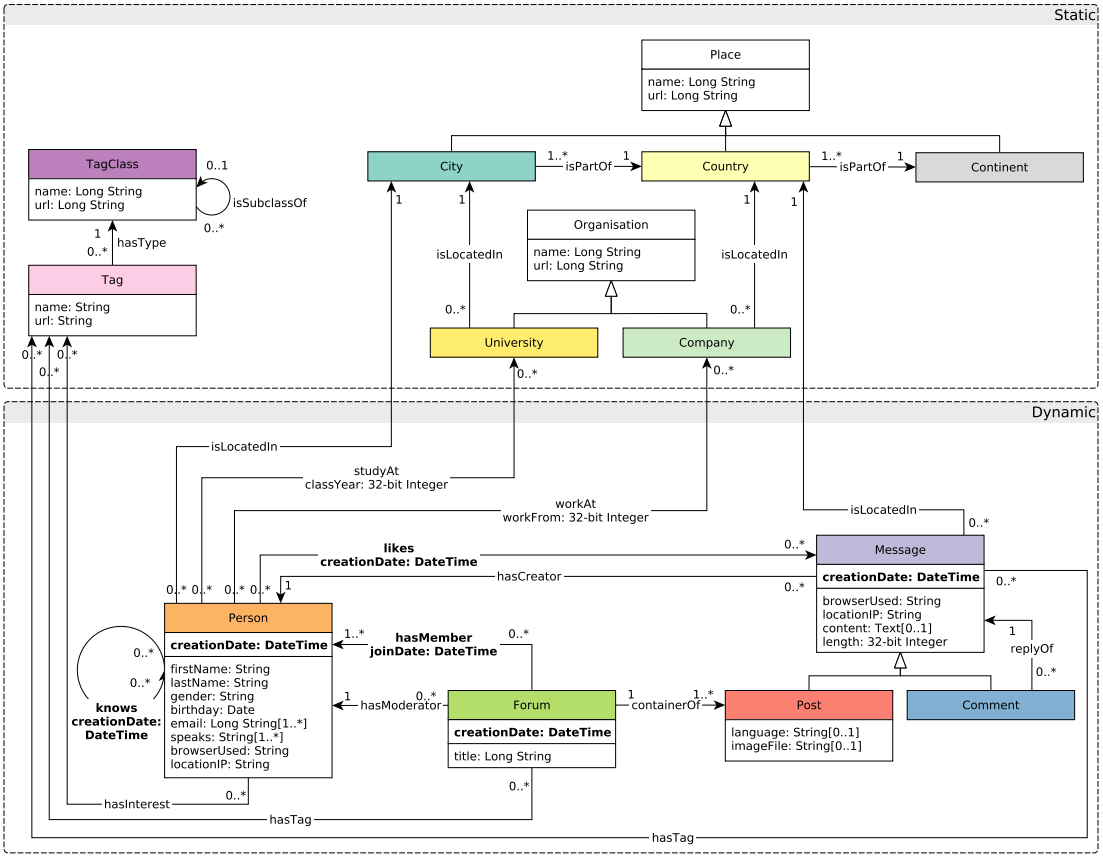
\includegraphics[scale=0.42]{img/ldbc-schema}
	\captionsetup{justification=centering}
	\caption{\gls{ldbc} Graph schema. (Obtained from LDBC SNB specification document v0.3.2)}
	\label{fig:ldbc-schema}
\end{figure}

\noindent \textbf{Datasets:} We use the \gls{ldbc}~\cite{ldbc} dataset generator to generate synthetic graph datasets on which we evaluate all our experiments. \gls{ldbc} is a highly popular, standard tool for benchmarking systems large social graphs. The generated social graph is highly structured which can be seen from the schema in Figure~\ref{fig:ldbc-schema}. Yet, the data is very sparse and have several unstructured edges and properties. Even though the real-world graph varies in the type of structures that exist in them, the \gls{ldbc} data is indicative that most of the graph data are indeed structured.

We generate the data at the scale factor of 100 (\gls{ldbc} 100) that consists of over 1.7 billion edges and 0.3 billion vertices.

\noindent \textbf{Query Workload:} Our query workload mainly consists of short path queries, like k-hop for $k=1,2,3$, with constraint evaluations and aggregations. We base our workloads on the \gls{ldbc} schema. We deliberately concentrate on using short queries as they serve as a stress test for evaluating access from the underlying storage. For instance, a simple 1-hop query tests more rigorously for access from adjacency lists than a query that involves filtering and aggregations. A possible extension could be to evaluate our work using the bigger workloads included in \gls{gdbms}.

\section{Compression in Adjacency Lists}
\label{exp:adjacency-list-exp}

We introduced several optimizations that can make use of the graph data's structure to drastically compact the representation of edges and vertices in the adjacency lists. In this experiment, we demonstrate the memory gains we derive from these optimizations on \gls{ldbc} 100 by recording the memory utilization of the adjacency lists across different configurations which we describe momentarily.

We create multiple configurations on GraphflowDB, each with a different set of optimizations. Below are the descriptions of the configurations we evaluate the memory usage on. Each configuration builds on top of previous in the list. 

\begin{enumerate}
	\item \texttt{GF-OLD:} This is our baseline configuration that represents edges and vertices in the adjacency list as 8-byte identifiers. All the edges are stored in the 2-level CSR structure and are not compressed.
	\item \texttt{+COLS}: Uses vertex property columns from single cardinality edge labels. 
	\item \texttt{+NEW-IDS}: Introduces the new vertex and edge identification scheme, i.e, the vertex ID is represented as a vertex label and an offset. For representing edge, we store a page-level.
	\item \texttt{+0-SUPR}: Implements leading 0 suppression in the components of vertex and edge IDs in adjacency lists.
	\item \texttt{+OMIT}: Omits to store neighbour vertex label and positional offsets of edge IDs wherever possible.
	\item \texttt{+NULL}: Implements prefixSum-based null compression on vertex property columns and adjacency list.
\end{enumerate}

\begin{table}
	\centering
	\bgroup
	\setlength{\tabcolsep}{8pt}
	\def\arraystretch{1.2}%  1 is the default, change whatever you need
	\begin{tabular}{ |c|c|c|c|c|c|c| } 
		\hline
		& \texttt{GF-OLD} & \texttt{+COLS} & \texttt{+NEW-IDS} & \texttt{+0-CMPRS} & \texttt{+OMIT}& \texttt{+NULL} \\ 
		\hline \hline
		Fwd. Adjacency Lists& 38.25 & 33.25 & 27.22 & 16.35 & 11.14 & 10.53 \\ 
		\hline
		Bwd. Adjacency Lists& 37.93 & 37.50 & 30.93 & 18.75 & 12.79 & 11.15 \\ 
		\hline
		Total& 76.18 & 70.75 & 58.15 & 35.10 & 23.93 & 21.68 \\ 
		\hline \hline
		\multirow{2}{80pt}{Bytes per edge}& 23.04 & 21.39 & 17.58 & 10.61 & 7.24 & 6.50 \\ 
		& & \textbf{1.08x} & \textbf{1.31x} & \textbf{2.17x} & \textbf{3.18x} & \textbf{3.55x} \\ 
		\hline
	\end{tabular}
	\egroup
	\captionsetup{justification=centering}
	\caption{Memory utilization (in GB) by Adjacency lists of \gls{ldbc} 100 accross configurations. }
	\label{tbl:mem1}
\end{table}

\begin{figure}
	\centering
	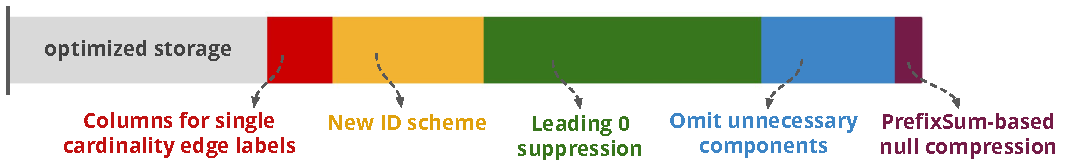
\includegraphics[scale=0.75]{img/opti-breakup}
	\captionsetup{justification=centering}
	\caption{Breakup of memory gains by applying different optimizations on Adjacency Lists of \gls{ldbc} scale factor 100 dataset.}
	\label{fig:opti-breakup}
\end{figure}

Table~\ref{tbl:mem1} shows the memory utiliation (in GB) by the adjacency lists for \gls{ldbc} 100 dataset accross different configurations, while Figure~\ref{fig:opti-breakup} gives the breakup of memory gain per optimization. Memory gain in \texttt{+COLS} is attributed to the fact that 8 out of 15 edge labels are single cardinality and stored in vertex columns in at least one direction. \texttt{+NEW-IDS} gains ({\raise.17ex\hbox{$\scriptstyle\sim$}}4 bytes per edge) by storing edges in much smaller size than 8 bytes, while \texttt{+OMIT} gains ({\raise.17ex\hbox{$\scriptstyle\sim$}}3 bytes per edge) from not storing edge's positional offsets and neighbour's vertex label for 10 out 15 edge labels. We do not see much benefits in \texttt{+NULL} ({\raise.17ex\hbox{$\scriptstyle\sim$}}0.75 bytes per edge) since empty adjacency lists are not too frequent in \gls{ldbc}. 

While storing edges in vertex columns benefits accessing the edge by avoiding indirection, \texttt{+NULL} incurs a small penalty but does not slow down the query significantly. \texttt{+COLS} and \texttt{+NULL} are evaluated in Sections~\ref{exp:single-cardinality} and ~\ref{exp:prefixSum} respectively. Unlike other \gls{gdbms}, we use fixed-length scheme for leading 0 suppression. This benefits us from not having to decode a particular value and hence, not suffer from performance loss. There will be marginal gains by copying lesser data from the adjacency lists (in case of \texttt{+OMIT} and \texttt{+NEW-IDS}) but we do not evaluate since the benefits are trivial.

Further, the memory utilization of \gls{ldbc} 300 (5.27B edges, 0.6B vertices) with our set of optimizations was 63.45GB. In all, we are able to scale the new GraphflowDB (with our new storage layer) to store up to 10.5B edges, along with vertex and edge properties, of \gls{ldbc} data on a single machine with 500GB of main memory. This is {\raise.17ex\hbox{$\scriptstyle\sim$}}15x increase in scalability compared to old GraphflowDB with unoptimized storage.

\section{Effectiveness of Single-Directional Property Pages}
\label{exp:property-pages}

In this experiment, we show the benefits of keeping the edge properties loosely grouped in single-directional property pages over edge columns that store the edge properties unordered. We also demonstrate that the keeping edge properties in property pages instead of single-directional property lists (which keeps properties tightly ordered by adjacency lists, but difficult to update) is a reasonable trade-off as we don't lose much performance but significantly win over edge columns. We configure  GraphflowDB to use the new ID scheme and build 3 versions for storing edge properties:

\begin{enumerate}
	\item \texttt{EDGE COLS:} Mimics the first solution in Section~\ref{sec:edge-cols-prop-lists}. In this configuration, the edge properties of label \texttt{knows} are stored in columns that are oblivious to the location of \texttt{knows} edges in either the forward or backward adjacency lists. 
	\item \texttt{PROP LISTS:} Edge properties of \texttt{knows} edges are stored in the single-directional (forward) property lists that mimics the forward adjacency lists. This solution is supposed to give localized reads for edge property while joining in the forward direction.
	\item \texttt{PROP PAGES:} Edge properties are stored in pages by combining $n=128$ property lists of the previous solution. This solution should still provide close-by reads when joining in the forward direction.
\end{enumerate}

\begin{table}
	\centering
	\bgroup
	\setlength{\tabcolsep}{8pt}
	\def\arraystretch{1.2}%  1 is the default, change whatever you need
	\begin{tabular}{ |c|c|c|c| } 
		\hline
		& \textbf{1-hop} & \textbf{2-hop} & \textbf{3-hop} \\
		\hline \hline
		\texttt{EDGE COLS}& 3.42 & 308.18 & 966.04\\ 
		\hline
		\multirow{2}{*}{\texttt{PROP LISTS}}& 1.03 & 125.65 & 372.44 \\ 
		& \textbf{3.32x} & \textbf{2.42x} & \textbf{2.59}\\ 
		\hline 
		\multirow{2}{*}{\texttt{PROP PAGES}} & 1.22 & 152.89 & 512.24 \\ 
		& \textbf{2.80x} & \textbf{2.03x} & \textbf{1.87} \\ 
		\hline \hline
		\texttt{PROP PAGES} vs \texttt{PROP LISTS} & 1.19x & 1.22x & 1.37x \\
		\hline
	\end{tabular}
	\egroup
	\captionsetup{justification=centering}
	\caption{Runtime (in sec) of k-hop queries for different configurations of edge property storage on \gls{ldbc} 100.}
	\label{tbl:mem2}
\end{table}

The workload comprises of 3 k-hop queries, $k=1,2,3$, on the \texttt{knows} edge label of the \gls{ldbc} schema (Figure~\ref{fig:ldbc-schema}) that compares each of the query edge's \texttt{creationDate} property to be greater than the previous edge in the query. 1-hop and 2-hop queries run for all vertices of \texttt{person} while we run 3-hop for only 25000 vertices owing to time constraints. For each query, we only consider the plan that matches vertices sequentially and joins only in the forward direction. This way we are ensured of cache locality in \texttt{PROP-LISTS} and \texttt{PROP-PAGES}.

Table~\ref{tbl:mem2} shows the performance of queries on 3 configurations. Clearly, the queries benefit from localizing of edge properties in the storage. The maximum gain which we get from property lists is 3.32x while that from property pages is 2.80x. The benefits decrease with the size of query because the last operators in a query plan flush the pages from which earlier operators read. However, both property lists and pages still guarantee benefits over unordered \texttt{EDGE COLS}. On the other hand, storing the edge properties in the update-friendly property pages only slightly degrades the performance of queries (1.19-1.37x). This depends on the value of $n$, i.e, the number of property lists that we put together on a page. The average number of \texttt{knows} edges per \texttt{person} vertex is {\raise.17ex\hbox{$\scriptstyle\sim$}}44 edges while $n=128$. A lower $n$ means that properties of edges in an adjacency lists appear closer in the page and hence, provide more localized reads.

\section{Vertex Property Columns for Single Cardinality Edges vs. 2-level CSR Adjacency Lists}
\label{exp:single-cardinality}

Storing single cardinality edges in vertex columns ensure two straight benefits, 1) direct access without indirection into CSR, and 2) does not need to store offsets of the CSR. We showed the memory gains of storing edges in vertex columns on \gls{ldbc} 100 in Section~\ref{exp:adjacency-list-exp}, though these benefits were cumulative of the entire adjacency lists. In this experiment we compare the performance of a query with single cardinality edges with respect to, 1) using vertex column vs 2-level CSR adjacency lists to store edges, and 2) if the end structure is null compressed or not. We explicitly test performance on the compressed data structures since having edge label cardinality \texttt{0..1} rather than \texttt{1} is common in real-world graphs. Hence, we create 4 configurations of GraphflowDB to run our queries on:

\begin{enumerate}
	\item \texttt{V-COL-UNC:} Single cardinality edge label edges are stored are in vertex columns and are not compressed. This is equivalent to \texttt{+OMIT} configuration in Section~\ref{exp:adjacency-list-exp}.
	\item \texttt{CSR-UNC:} Single cardinality edge label edges are stored in 2-level CSR adjacency lists and are not compressed.
	\item \texttt{V-COL-C:} PrefixSum-based \texttt{NULL} Compressed version of \texttt{V-COL-UNC}. This is equivalent to \texttt{+NULL} configuration in Section~\ref{exp:adjacency-list-exp}.
	\item \texttt{CSR-C:} PrefixSum-based \texttt{NULL} Compressed version of \texttt{CSR-UNC}.
\end{enumerate}

The workload consists of simple 3 k-hop queries, $k=1,2,3$, on the \texttt{replyOf} edge between \texttt{comment} vertices in the \gls{ldbc} schema. The \texttt{replyOf} edge label has \texttt{n-1} cardinality, hence, we keep the forward edges as a special property of \texttt{comment} vertex label. Moreover, our workload queries do not do any predicate evaluation and the final output of the query is an aggregated count. This assures that \texttt{JOIN} operation in the query plan is the only dominant operation. Again, for each query, we evaluate only on the plan that matches the vertices sequentially and joins in the forward direction.

\begin{table}
	\centering
	\begin{subtable}{1\textwidth}
		\centering
		\bgroup
		\setlength{\tabcolsep}{8pt}
		\def\arraystretch{1.2}%  1 is the default, change whatever you need
		\begin{tabular}{ |c|c|c|c|c| }
			\hline
			& \textbf{1-hop} & \textbf{2-hop} & \textbf{3-hop} & \textbf{Memory (in MB)} \\ 
			\hline \hline
			\texttt{CSR-UNC}& 7.03 & 9.13 & 9.60 & 1266.56 \\ 
			\hline
			\multirow{2}{*}{\texttt{V-COL-UNC}}& 4.34 & 5.80 & 5.85 & 839.93 \\ 
			& \textbf{1.62x} & \textbf{1.57x} & \textbf{1.64x} & \textbf{1.51x} \\ 
			\hline
		\end{tabular}
		\egroup
		\captionsetup{justification=centering}
		\caption{Uncompressed}
		\label{tbl:s1}
	\end{subtable}
	\begin{subtable}{1\textwidth}
		\centering
		\bgroup
		\setlength{\tabcolsep}{8pt}
		\def\arraystretch{1.2}
		\begin{tabular}{ |c|c|c|c|c| } 
			\hline
			& \textbf{1-hop} & \textbf{2-hop} & \textbf{3-hop} & \textbf{Memory (in MB)} \\ 
			\hline \hline
			\texttt{CSR-C}& 7.78 & 10.40 & 11.23 & 905.23 \\ 
			\hline
			\multirow{2}{*}{\texttt{V-COL-C}}& 5.23 & 8.28 & 8.41 & 478.86 \\ 
			& \textbf{1.49x} & \textbf{1.26x} & \textbf{1.34x} & \textbf{1.89x} \\ 
			\hline
		\end{tabular}
		\egroup
		\captionsetup{justification=centering}
		\caption{Null Compressed}
		\label{tbl:s2}
	\end{subtable}
	\captionsetup{justification=centering}
	\caption{Vertex property columns vs. 2-level CSR adjacency lists for storing single cardinality edges: Query runtime (in sec) and Memory usage (in MB)  }
\end{table}

Tables~\ref{tbl:s1} and ~\ref{tbl:s2} shows the result of queries on uncompressed and null compressed configurations respectively. 	We get the maximum speed up of 1.62x in uncompressed variants, while its lesser for compressed couterparts with the maximum 1.49x. The last column of the tables report the size of the adjacency lists or vertex column storing \texttt{replyOf} edges. Here, vertex column uses half as much space as adjacency lists, when the data is kept compressed. In \gls{ldbc} 100, out of {\raise.17ex\hbox{$\scriptstyle\sim$}}220M \texttt{comment} vertices, approx. 50\% have empty forward adjacency list, i.e, do not have an outward \texttt{replyOf} edge. This is reflected in vertex columns between \texttt{V-COL-UNC} and \texttt{V-COL-C}, as the memory reduces to half (839.93MB vs 478.86MB), unlike their CSR counterparts that stores offsets as extra and thus, compression reduces memory by only 25\%.

\section{Effectiveness of PrefixSum-based Null Compression Technique}
\label{exp:prefixSum}

PrefixSum-based null compression technique is used in our system to compress both, sparse columns and empty adjacency lists. We evaluate our technique in 2 settings, 1) Storage and random access efficacy against uncompressed and vanilla NULL compressed columns, and 2) query performance on compressed and uncompressed vertex columns and adjacency lists.

\subsection{Stress Test} 

\begin{figure}
	\hspace*{-25pt}
	\begin{subfigure}{0.55\textwidth}
		\centering
		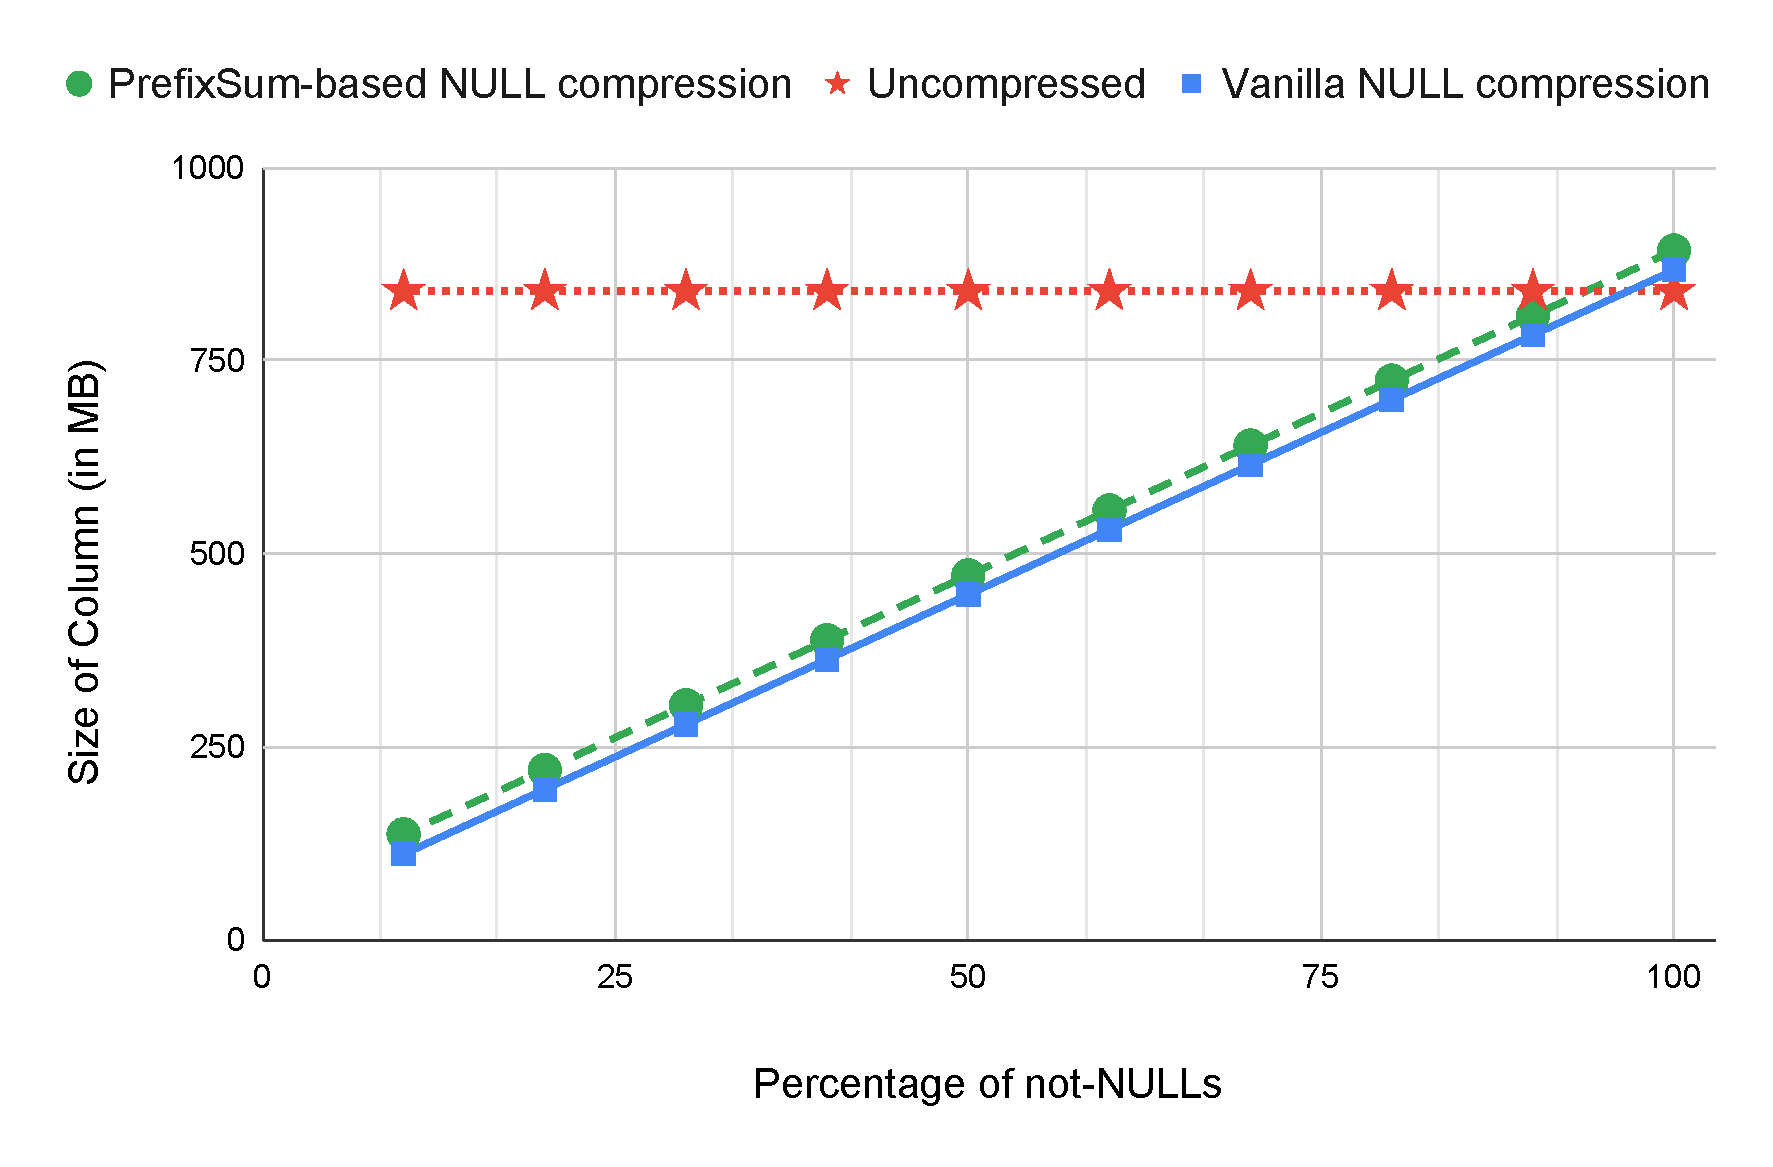
\includegraphics[scale=0.30]{img/pref-space}
		\captionsetup{justification=centering}
		\caption{Memory usage}
		\label{fig:pref-space}
	\end{subfigure}
	\begin{subfigure}{0.55\textwidth}
		\centering
		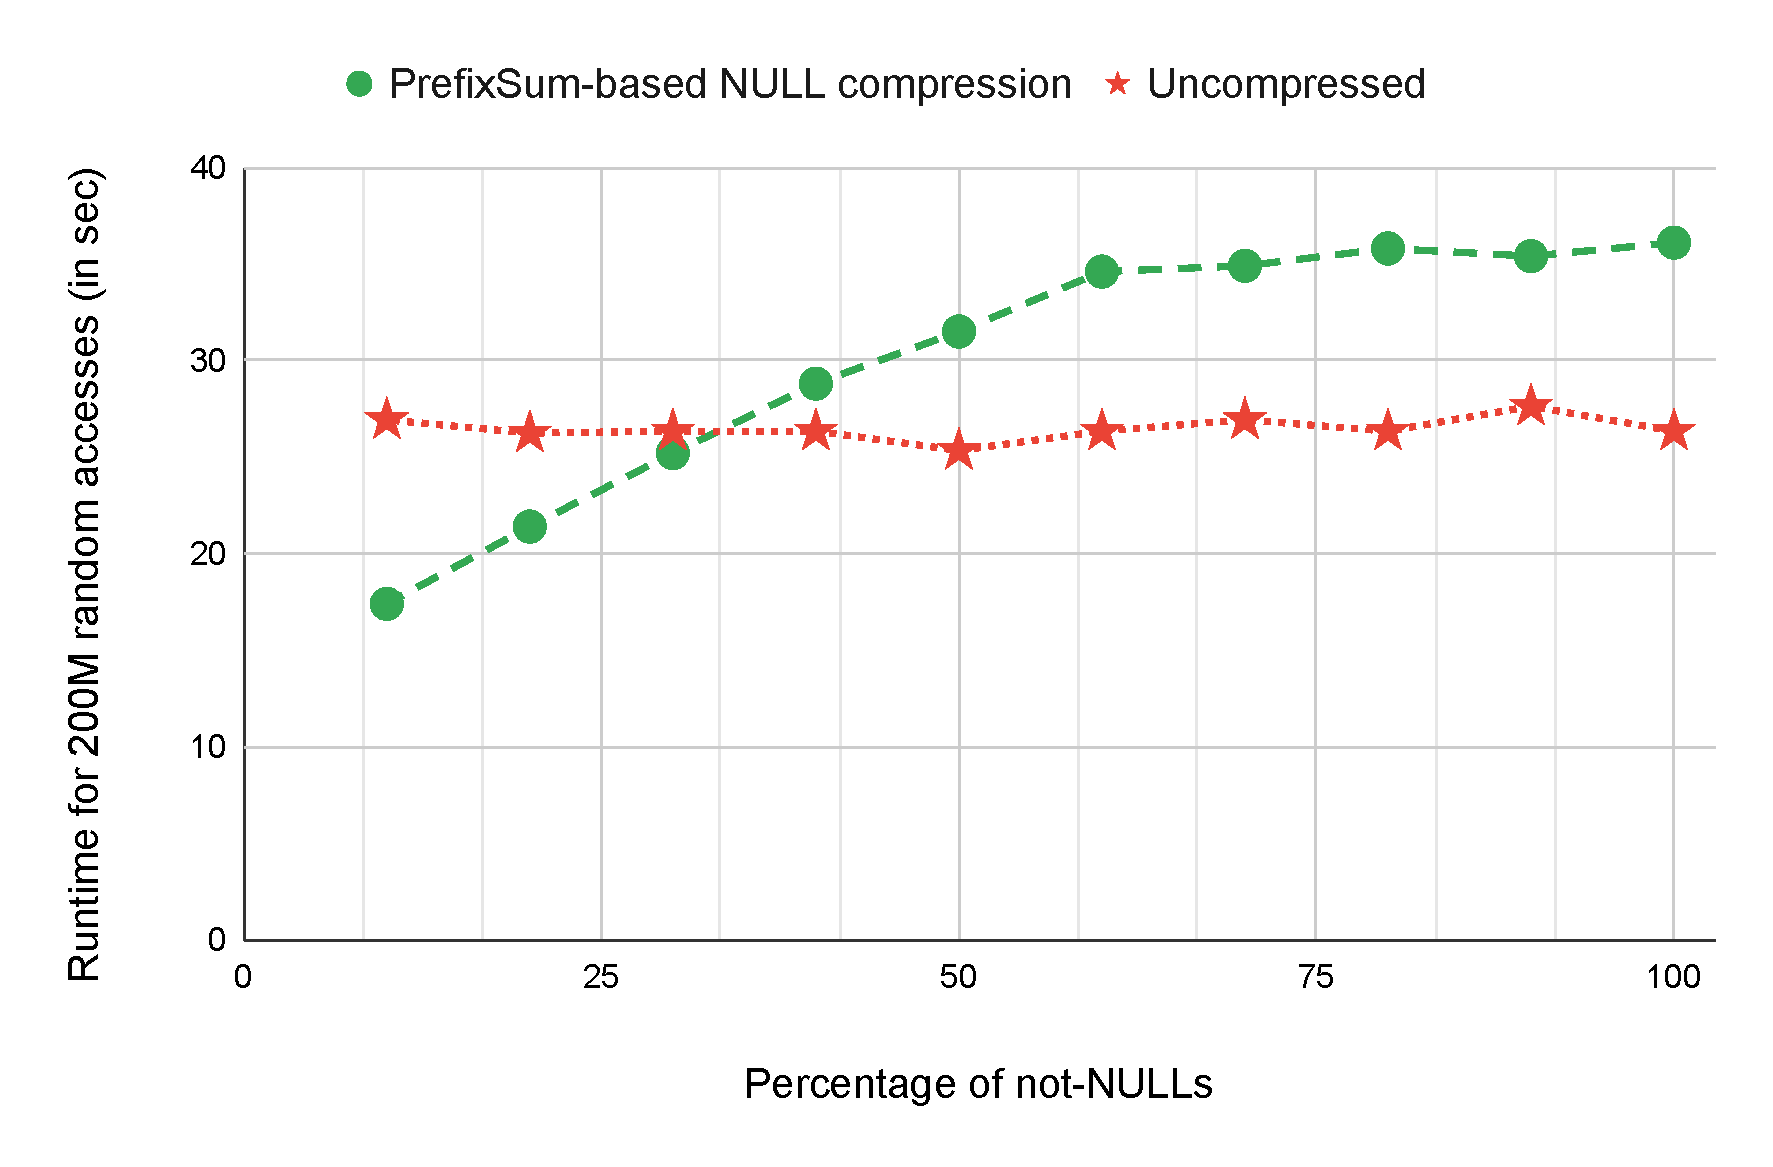
\includegraphics[scale=0.30]{img/pref-perf}
		\captionsetup{justification=centering}
		\caption{Performance on random accesses}
		\label{fig:pref-perf}
	\end{subfigure}
	\captionsetup{justification=centering}
	\caption{Memory and performance on random accesses for Uncompressed, prefixSum-based NULL compressed and vanilla NULL compressed columns.}
	\label{fig:pref-stress}
\end{figure}

The goal of this experiment is to compare uncompressed, prefixSum-based null compressed and vanilla null compressed (as implemented in ~\cite{abadi-sparse-col}) columnar data-structure for memory usage and performance on random reads. For this, we use the \texttt{creationDate} property of 220M \texttt{comment} vertices in \gls{ldbc} 100 and create multiple versions of it, each with different \%age of non-\texttt{NULL} values. On each version, we do the necessary compression and measure the time taken to do 200M access to random locations in the that column. 

Figures~\ref{fig:pref-space} and~\ref{fig:pref-perf} shows memory usage and performance on 200M random read queries respectively, for uncompressed, prefixSum-based \texttt{NULL} compressed and vanilla \texttt{NULL} compressed column of \texttt{creationDate} property of \texttt{comment} vertex label. We omit the performance number of vanilla \texttt{NULL} compression as they were significantly higher than the other two ($>$20x). Our prefixSum-based \texttt{NULL} compression technique is only marginally over vanilla \texttt{NULL} comression in memory usage (we take 2-bit for each element vs. 1-bit overhead in vanilla compression). However, introducing prefixSums and map lookups, in place of iterations over bit-strings, makes the performance of random access comparable on prefixSum-based \texttt{NULL} compressed column comparable to uncompressed (1.38x slower at worst). In fact, our compression comes out to be faster than uncompressed for very sparse columns ($<30$ non-\texttt{NULL} values). This is because testing for \texttt{NULL} at a location is a constant time operation.

\subsection{Query Performance}

Tables~\ref{tbl:s1} and~\ref{tbl:s2} already compares reading edges from compressed and uncompressed adjacency lists and vertex columns. Reading edges from CSR adjacency lists and vertex columns that are \texttt{NULL} compressed by our technique are on average 1.14x and 1.3x slower than their uncompressed variant respectively. However, for 50\% \texttt{NULL} values, they gain 50\% and 25\% in storage respectively. 

\begin{table}
	\centering
	\bgroup
	\setlength{\tabcolsep}{8pt}
	\def\arraystretch{1.2}%  1 is the default, change whatever you need
	\begin{tabular}{ |c|c|c|c| } 
		\hline
		& \textbf{1-hop} & \textbf{2-hop} & \textbf{3-hop} \\
		\hline \hline
		\texttt{V-COL-UNC}& 12.78 & 14.47 & 14.95\\ 
		\hline
		\multirow{2}{*}{\texttt{V-COL-C}}& 14.65 & 16.00 & 16.98 \\ 
		& \textbf{1.15x} & \textbf{1.11x} & \textbf{1.14x}\\ 
		\hline  
	\end{tabular}
	\egroup
	\captionsetup{justification=centering}
	\caption{Runtime (in sec) of k-hop queries on compressed and uncompressed vertex column on \gls{ldbc} 100.}
	\label{tbl:s3}
\end{table}

We next evaluate accessing vertex properties from compressed and uncompressed vertex columns on configurations \texttt{V-COL-C} and \texttt{V-COL-UNC} respectively. Edge storage is not compressed in these configurations. We run a workload derived from that in Section~\ref{exp:single-cardinality} consisting of k-hop queries over \texttt{replyOf} edges. These queries are extended to include a condition that a \texttt{comment} $b$ is made on another \texttt{comment} $a$ such that $b$ has a \texttt{creationDate} that is within $\delta$ timespan of $a$'s. Table~\ref{tbl:s3} shows the numbers from the experiment which suggest that using compressed storage only slows down the query by 1.14x which is a reasonable trade-off when compared to compact storage. We can expect the slow down factor to be always intermediary less than those we reported in the stress test.

\section{List-based Processing vs. Volcano-styled Query Execution}
\label{exp:list-based}

We compare list-based query processing to the conventional volcano-styled processing on several path queries.





















